\documentclass{thureport}
% =============================================
% Part 1 Edit the info
% =============================================

\newcommand{\major}{软件71}
\newcommand{\name}{骆炳君}
\newcommand{\stuid}{2017013573}
\newcommand{\newdate}{2019-4-1}
\newcommand{\newtitle}{压电元件导纳圆的测量及互感耦合电路特性研究}
\def\celsius{{\ensuremath{^\circ\hspace{-0.09em}\mathrm{C}}}}

% =============================================
% Part 1 Main document
% =============================================
\begin{document}
\thispagestyle{empty}
\begin{figure}[h]
	\begin{minipage}{0.65\linewidth}
		\centerline{
\includegraphics[width=\linewidth]{head.jpg}}
	\end{minipage}
	\hfill
	\begin{minipage}{.3\linewidth}
		\raggedleft
		\begin{tabular*}{.8\linewidth}{ll}
			班级: & \underline\major   \\
			姓名: & \underline\name    \\
			学号: & \underline\stuid   \\
			日期: & \underline\newdate
		\end{tabular*}
	\end{minipage}
\end{figure}

\begin{table}[!htbp]
	\centering\large
	实验名称: \underline\newtitle
\end{table}

\tableofcontents
% =============================================
% Part 2 Main document
% =============================================
\newpage

\section{实验目的}
\begin{clause}
	\item 测量压电元件的导纳,即测量阻抗,可提供该元件与所在电路之间的阻抗匹配数据.
	\item 通过测量压电元件或压电换能器的导纳圆可以得到其发射效率.
	\item 学习利用示波器测量交流阻抗的方法.
\end{clause}

\section{数据处理}
\subsection{压电元件导纳圆的测量}
函数信号发生器$V=8V$,$R=2.98\Omega$.

由附录中的导纳圆图可以得出
$$D=108.520ms,\ f_1=88.94kHz,\ f_2=89.93kHz$$

测得数据如下表:
\begin{table}[htbp]
    \centering
      \begin{tabular}{|c|c|c|c|c|}
      \hline
            & 频率($kHz$) & 相差($\mu s$) & $U$($V$) & $U_I$($V$) \bigstrut\\
      \hline
      1     & 91.574  & 2.60  & 3.78  & 0.090  \bigstrut\\
      \hline
      2     & 91.170  & 2.24  & 3.38  & 0.112  \bigstrut\\
      \hline
      3     & 89.163  & 0.80  & 0.78  & 0.222  \bigstrut\\
      \hline
      4     & 89.117  & 0.44  & 0.71  & 0.224  \bigstrut\\
      \hline
      5     & 89.096  & 0.08  & 0.70  & 0.229  \bigstrut\\
      \hline
      6     & 89.063  & -0.28  & 0.70  & 0.226  \bigstrut\\
      \hline
      7     & 89.029  & -0.64  & 0.74  & 0.222  \bigstrut\\
      \hline
      8     & 88.997  & -1.00  & 0.82  & 0.222  \bigstrut\\
      \hline
      9     & 88.952  & -1.36  & 0.93  & 0.226  \bigstrut\\
      \hline
      10    & 88.886  & -1.72  & 1.14  & 0.224  \bigstrut\\
      \hline
      11    & 88.764  & -2.08  & 1.54  & 0.218  \bigstrut\\
      \hline
      12    & 88.438  & -2.44  & 2.44  & 0.192  \bigstrut\\
      \hline
      \end{tabular}%
    \label{tab:addlabel}%
  \end{table}%

由
$$R+R_1=\frac{1}{D},\ L_1=\frac{R_1+R}{\omega_2-\omega_1}$$

得
$$R_1=\frac{1}{D}-R=\frac{1}{0.108520}-2.98=6.23(\Omega)$$

$$L_1=\frac{1}{2\pi D(f_2-f_1)}=\frac{1}{2\pi\times108.520\times(89.93-88.94)}=1.481\times10^{-3}(H)$$

$$C_1=\frac{1}{\omega_1\omega_2L_1}=\frac{1}{4\pi^2f_1f_2L_1}=\frac{1}{4\pi^2\times89.93\times88.94\times1.481\times10^3}=2.138\times10^{-9}(F)$$

$$C_0=\frac{\overline{AC}}{2\pi\sqrt{f_1f_2}}=\frac{1.239\times10^{-3}}{2\pi\sqrt{89.93\times88.94\times10^6}}=2.205\times10^{-9}(F)$$

机械品质因素
$$Q_m=\frac{1}{R_1}\sqrt{\frac{L_1}{C_1}}=\frac{1}{6.23}\sqrt{\frac{1.481\times10^{-3}}{2.138\times10^{-9}}}=133.59$$

\subsection{示波器研究互感耦合电路特性}
$M=,\ L_2=,\ f=5kHz,\ \omega=2\pi f=3.1416\times10^4rad/s$

测得数据如下表:

由$R_2=\infty$时$\Delta R=0$得,$R=(\Omega)$

由表中数据可得,$\Delta R_{1max}=\Omega$

其理论值为$$\Delta R_{1max}=\frac{2\pi fM^2}{2L_2}=\frac{2\pi\times\times}{2\times}=(\Omega)$$

相对偏差为$\frac{-}{}\times100\%=\%$
\section{实验小结}
本实验利用铜电阻温度传感器和硅压阻式差压传感器,采取水浴加热的方法测量空气(可近似为理想气体)在定容条件下的多组压强、温度数据,并进行直线拟合,在误差允许的范围内验证了理想气体查理定律,测得了空气相对压力系数,取得了较好的实验结果.

\section{思考题}
\subsection*{1.}
压电元件的共振就是加在压电元件两端的交流电频率与其固有频率相等从而使元件得振幅达到最大的现象.判断方法为$U$与$U_I$同相且$U_I$振幅最大.

\subsection*{2.}
当$U_I$领先$U$时,$\varphi_{U_I}>\varphi_{U}$,$\tau>0$;当$U$领先$U_I$时,$\varphi_{U_I}<\varphi_{U}$,$\tau<0$.

\subsection*{3.}
由于导纳圆图中的两个圆几乎重合,可认为此时$(g_1,b_1)=(g,b)=(\frac{U_I}{UR}cos\frac{2\pi\tau}{T},\frac{U_I}{UR}sin\frac{2\pi\tau}{T})$,在$\tau$为等差级数时实验点也将均匀分布在导纳圆上.

\subsection*{4.}
$R$既不能太大也不能太小.$R$取大了会使电流减小,压电元件的分压减小,测量得出的数值过小,效果不明显.

\clearpage
\section{拟合曲线}
\begin{figure}[h]
	\centering
	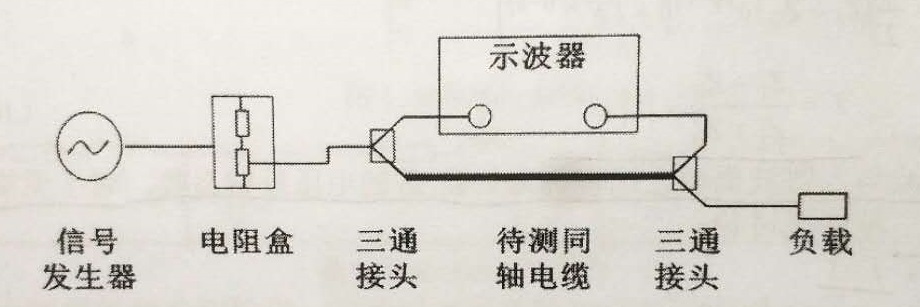
\includegraphics[width=0.9\linewidth]{figure1.jpg}
\end{figure}

\clearpage
\section{原始数据表格}
\clearpage

\end{document}